\section{Results}
All numbers are means over the 300 SCMs and three seeds unless stated otherwise; the designated held-out family (layered) is marked $^\dagger$. The outcome is learnable but not trivially so: XGBoost and the MLP reach a mean test $R^2$ of $0.63$ and $0.62$ (range $0.10$--$0.93$) against an oracle $R^2$ of $f^*$ of $0.67$ (range $0.23$--$0.94$).

\subsection{Where explanation error comes from}
\TableDecomposition
Table~\ref{tab:decomp} and Fig.~\ref{fig:decomp} give the decomposition. Three observations hold for both models and all explainers.

\emph{The estimand gap dominates.} With the true function and exact Shapley values the importance shares are already $0.31$ ($L_2$) away from the shares of the causal effect, and the ranking differs by $0.37$ in $1-\tau_b$ units. Model misfit adds $0.09$ (XGBoost) to $0.14$ (MLP) in share space. The approximation error of the explainer itself is an order of magnitude smaller for KernelSHAP ($0.003$--$0.007$)---its coalition budget of $2^d/4$ is enough---and modest for LIME ($0.06$). Permutation importance, a global, loss-based measure, is the only explainer whose own error ($0.15$--$0.17$) rivals model misfit.

\emph{Better explainers do not help with the causal reading.} The rank error against $\Tau$ is $0.43$ for exact SHAP of the fitted model, $0.43$ for TreeSHAP and KernelSHAP, $0.44$--$0.46$ for LIME and $0.43$ for permutation importance; top-$k$ recovery of the causal drivers is $0.89$--$0.91$ for every method. Replacing a sampled explainer by an exact one changes the third term of~\eqref{eq:decomp} and leaves the ranking essentially where it was.

\emph{Misfit is not additive with the gap.} The MLP has the larger model misfit yet the smaller total share error ($0.23$ vs $0.26$ for XGBoost with exact SHAP). A smoother fitted surface spreads some credit onto correlated upstream features that the true function ignores, which happens to move the attribution \emph{towards} the total effect. This is a reminder that the component norms are reported separately for a reason: the vectors telescope, their magnitudes do not add.

\begin{figure}[t]
\centering
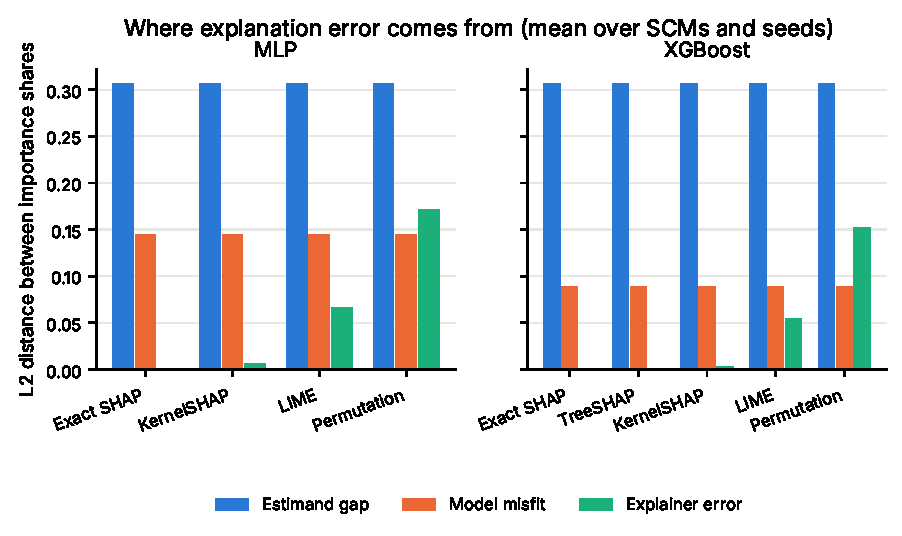
\includegraphics[width=\columnwidth]{fig_error_decomposition_share}
\caption{Share-space error components per explainer and model, mean over SCMs and seeds. The estimand gap (blue) is identical across explainers by construction; the explainer's own error (green) is the smallest term except for permutation importance.}
\label{fig:decomp}
\end{figure}

\subsection{The estimand gap depends on the causal structure}
\TableGapByFamily
\begin{figure}[t]
\centering
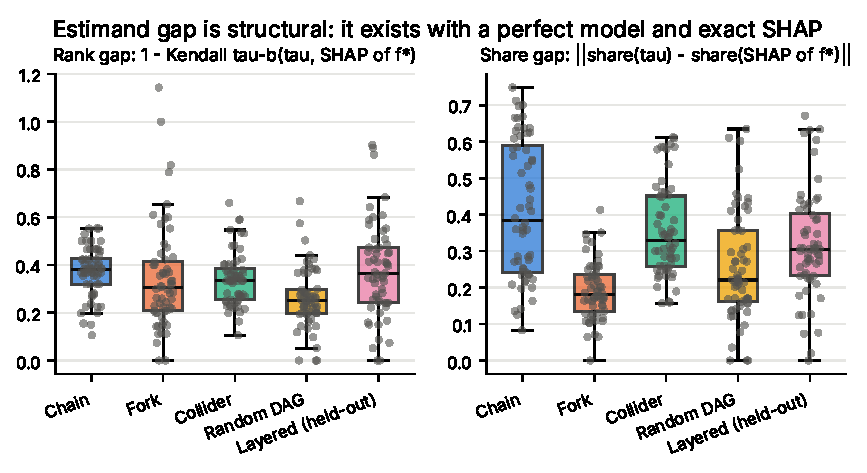
\includegraphics[width=\columnwidth]{fig_estimand_gap_by_family}
\caption{Estimand gap per graph family, one point per SCM (rank space left, share space right). The gap exists for a perfect model and an exact explainer; its size is set by the graph.}
\label{fig:gap}
\end{figure}
Table~\ref{tab:gap} and Fig.~\ref{fig:gap} break the gap down by family. It is largest in share terms for chain-mediation worlds ($0.41$), where on average $38\%$ of the total causal effect sits on features that act on $Y$ only through other features; the true function---and therefore exact SHAP of it---gives them exactly zero, and KernelSHAP and LIME on the fitted models give them $15\%$ and $11\%$. The confounded-fork family shows the opposite failure: non-parents of $Y$ carry only $8\%$ of the causal effect but receive $10\%$ of KernelSHAP's credit, because the fitted models use the confounded proxies. Feature-collider ($0.36$) and layered$^\dagger$ ($0.32$) worlds follow; Erd\H{o}s--R\'enyi DAGs, which have many direct parents of $Y$, have the smallest gap ($0.26$ share, $0.26$ rank). In rank space the ordering is flatter ($0.26$--$0.38$) because a few mediated features with zero attribution already produce several discordant pairs regardless of family. Total rank error of the fitted-model explainers follows the same ordering (chain $0.53$, collider $0.45$, layered$^\dagger$ $0.44$, fork $0.39$, random DAG $0.37$). Every one of the 300 SCMs has a non-zero rank gap.

\subsection{Predicting the error without ground truth}
\TableDiagnosticShare
\TableDiagnosticRank
Tables~\ref{tab:diag_share} and~\ref{tab:diag_rank} report the diagnostic for the two headline targets under the three protocols; Table~\ref{tab:logfo} and Fig.~\ref{fig:logfo} break the LOGFO result down by held-out family.

\emph{Share error is predictable and transfers.} For the share-error target the GBM meta-model reaches a pooled Spearman $\rho$ of $0.65$ ($R^2 = 0.53$) on unseen SCMs from seen families, $0.52$ ($R^2 = 0.33$; bootstrap 95\% CI $[0.43, 0.62]$) under leave-one-graph-family-out, and $0.48$ on the designated held-out layered family. The AUROC for flagging explanations whose share error exceeds the training median is $0.82$, $0.76$ and $0.75$ respectively. All three meta-models behave alike (random forest $0.54$, ridge $0.47$ under LOGFO), so the signal is not an artefact of one learner. Family by family (Table~\ref{tab:logfo}), the meta-model is the best method on every held-out family with $\rho$ between $0.29$ (fork) and $0.81$ (collider) and AUROC between $0.69$ and $0.88$. The best single-signal baseline is test error ($\rho = 0.36$ LOGFO), followed by explainer disagreement ($0.23$); correlation-only, maximum VIF and the constant are at or below zero.

\emph{Rank error is much harder.} For $1 - \tau_b$ the same meta-model reaches $\rho = 0.34$ in-distribution but only $0.22$ under LOGFO and $0.20$ on the layered family, with $R^2$ near zero. Only the disagreement and stability baselines carry any signal for this target ($0.19$ and $0.15$), and the meta-model's gain over them is not significant (Section~\ref{sec:tests}). With at most ten features, Kendall $\tau_b$ takes few distinct values and is dominated by which features receive exact zeros---a structural fact that, as the next section shows, the observables barely see.

\TableLogfoFamily
\begin{figure}[t]
\centering
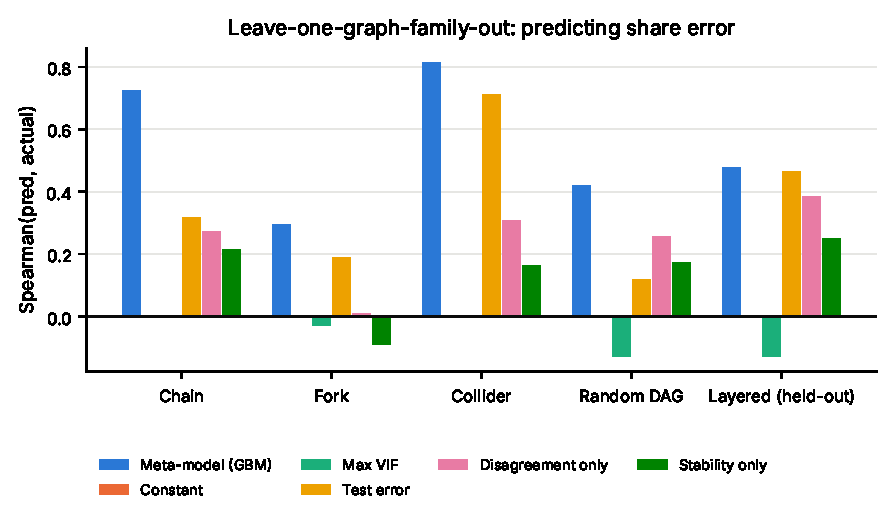
\includegraphics[width=\columnwidth]{fig_logfo_spearman_total_error_share_l2}
\caption{Leave-one-graph-family-out: Spearman correlation between predicted and actual share error on each held-out family, for the GBM meta-model and the single-signal baselines.}
\label{fig:logfo}
\end{figure}
\begin{figure}[t]
\centering
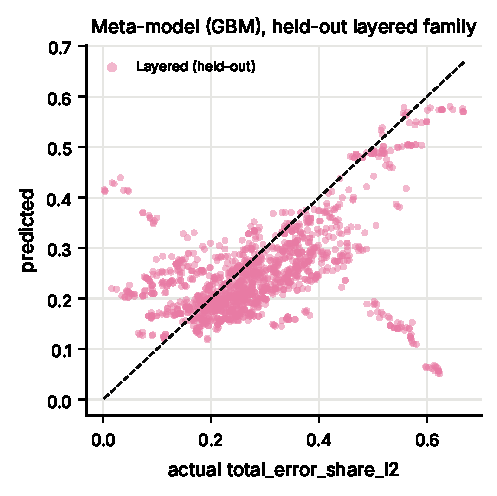
\includegraphics[width=0.8\columnwidth]{fig_pred_vs_actual_designated_split_meta_gbm_total_error_share_l2}
\caption{Predicted vs actual share error on the held-out layered family for the GBM meta-model trained on the four training families.}
\label{fig:pva}
\end{figure}

\subsection{Which part of the error is predictable}
\TableComponents
\begin{figure}[t]
\centering
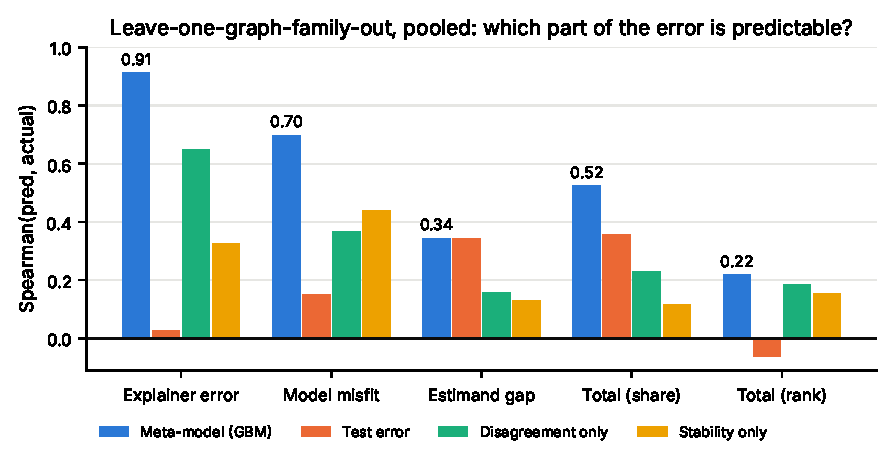
\includegraphics[width=\columnwidth]{fig_component_predictability_logfo_spearman}
\caption{Pooled LOGFO Spearman $\rho$ when each component of the decomposition is the prediction target. The explainer's and the model's contributions are predictable; the structural estimand gap is not.}
\label{fig:components}
\end{figure}
Table~\ref{tab:components} and Fig.~\ref{fig:components} repeat the experiment with each component of~\eqref{eq:decomp} as the target. The ordering is stark. \emph{Explainer error} is almost perfectly predictable ($\rho = 0.91$, $R^2 = 0.98$ under LOGFO): disagreement between explainers run on the same model accounts for most of it on its own ($\rho = 0.65$), with the LIME indicator and sign consistency next. \emph{Model misfit} is well predicted ($\rho = 0.70$, $R^2 = 0.59$), and here the combination matters: test error alone gives $0.15$ and disagreement alone $0.37$, while the meta-model's most important inputs are the disagreement between the XGBoost and MLP attributions, the model indicator, the top-1 share and the seed stability. The \emph{estimand gap}, the largest component, is the least predictable ($\rho = 0.34$, $R^2 = 0.11$), and the meta-model does no better than test error alone ($0.34$); on the layered family it is worse ($0.38$ vs $0.49$). What signal exists comes from the mean feature--outcome correlation and mutual information and from attribution concentration.

The reading is simple. The two components a practitioner could act on---fit the model better, use a better explainer---are the ones the observables reveal. The component that dominates the total is set by which correlated inputs are causes, mediators or proxies of $Y$, and nothing in the observational data, the fitted model or the attributions distinguishes those cases. Because the gap dominates, the total share error is only moderately predictable and the rank error, which is almost entirely gap, hardly at all.

\subsection{Is the gain over the baselines real?}
\label{sec:tests}
\TablePairedTests
Table~\ref{tab:tests} gives the paired comparisons for the share-error target. Under LOGFO the meta-model beats every baseline: against the strongest, test error, the Spearman gain is $0.17$ with a 95\% cluster-bootstrap interval of $[0.08, 0.25]$, the MAE gain is $0.019$ $[0.012, 0.026]$, the Wilcoxon signed-rank test on per-SCM errors gives $p < 0.001$, and the meta-model has the lower error on $65\%$ of SCMs; against the remaining baselines the gains are larger and all intervals exclude zero. On the layered family alone the picture is weaker: the meta-model beats the constant, correlation, VIF, sample-size and stability baselines ($p \le 0.05$) but is indistinguishable from test error ($\Delta\rho = 0.02$ $[-0.28, 0.28]$, $p = 0.62$) and from disagreement ($p = 0.12$); with 60 SCMs in one family the intervals are wide. For the rank-error target the meta-model's gains over disagreement and stability are not significant under any protocol.

\subsection{Which observables carry the signal}
\TableFeatureImportance
\begin{figure}[t]
\centering
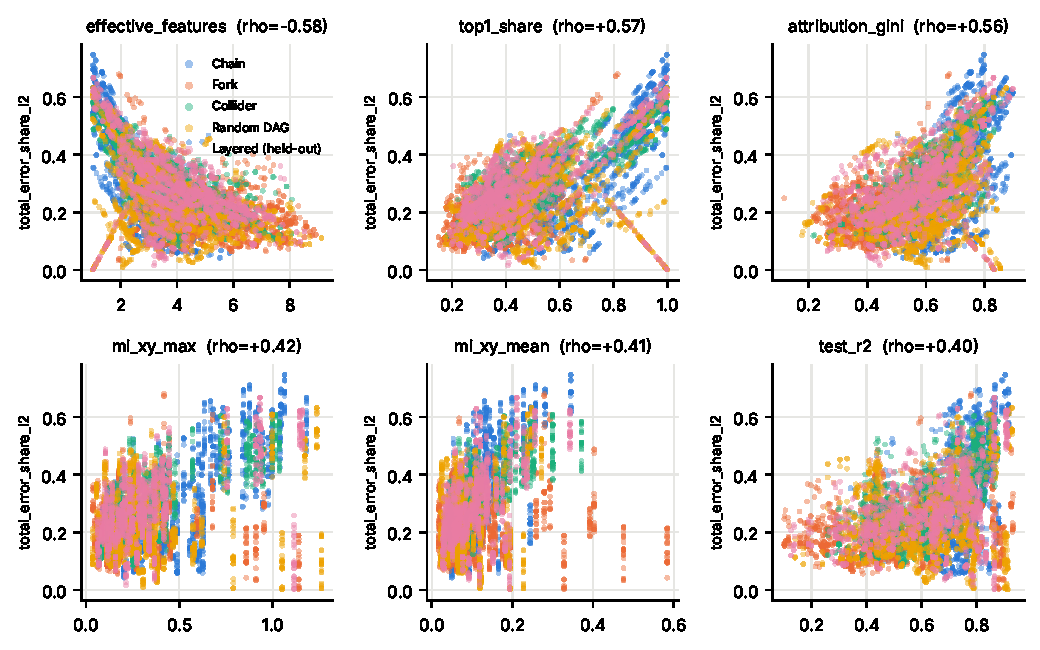
\includegraphics[width=\columnwidth]{fig_observables_vs_total_error_share_l2}
\caption{The six observables most correlated with the share error, one point per explanation, coloured by graph family (Spearman $\rho$ in the panel titles).}
\label{fig:obs}
\end{figure}
Table~\ref{tab:fi} lists the permutation importances of the meta-model trained on the training families and scored on the layered family, and Fig.~\ref{fig:obs} shows the strongest univariate relations. Two groups of observables matter. \emph{Concentration}: explanations that put their mass on few features are far from the causal shares (effective number of features $\rho = -0.58$; top-1 share $+0.57$; Gini $+0.56$). In this benchmark the causal effect is spread along chains and forks while $f^*$, and any model that fits it, concentrates on the direct parents of $Y$. \emph{Feature--outcome association and fit}: the mean feature--outcome $|r|$ has the largest permutation importance ($0.19$), with mutual information with $Y$ ($0.42$ univariate), test $R^2$ ($+0.40$) and cross-model agreement ($+0.39$) close behind. The sign of the fit relation is not the naive one: better-fit outcomes are those with a few dominant direct parents, which is exactly where exact SHAP concentrates credit that the causal effect spreads upstream. Disagreement between explainers ($\rho = 0.34$) and the stability measures add smaller but consistent contributions; maximum VIF, the quantity most often checked in practice, is almost uninformative on its own ($\rho = -0.13$ to $0.05$ across protocols).

\subsection{Ranking SCMs for a fixed explainer}
\TableByMethod
A large part of the variance in error is between explanation methods, which the model and explainer indicators capture trivially. Table~\ref{tab:bymethod} removes that part by scoring predictions within each (model, explainer) subset. The meta-model still ranks SCMs by share error with $\rho = 0.45$--$0.55$ under LOGFO, against $0.27$--$0.47$ for the test-error baseline; the advantage is largest for LIME ($0.45$ vs $0.27$--$0.31$), whose own error is well captured by the disagreement observables, and smallest for permutation importance, whose share error is dominated by its global, loss-based definition.
